\section{ResNet}
Another expansion built on CNNs is ResNet (Residual Network) \cite{resnet2016}, which succeeded in tackling issues with very deep networks. The general consensus was, the deeper the network is, the better performance it gives. However, it was observed, that training error for deeper networks gets higher than for their less deep counterparts. 

The degradation problem is caused by vanishing/exploding gradients. During backpropagation, multiplication of small (<1) and big (>1) numbers occurs. In deep networks, the multiplication takes place many times, causing it to get smaller and smaller until it vanishes or bigger and bigger until it blows up.

This problem can be solved by introducing residual blocks \ref{fig:res-block}. A skip connection is used to allow \textit{x} to be added to the output of later layers. This means, if vanishing gradient occurs, the network can be saved by ``going back'' to the previous layers. \ref{fig:resnet} shows a plain network and its counterpart (ResNet) with skip connections.

\begin{figure}[ht!]
    \centering
    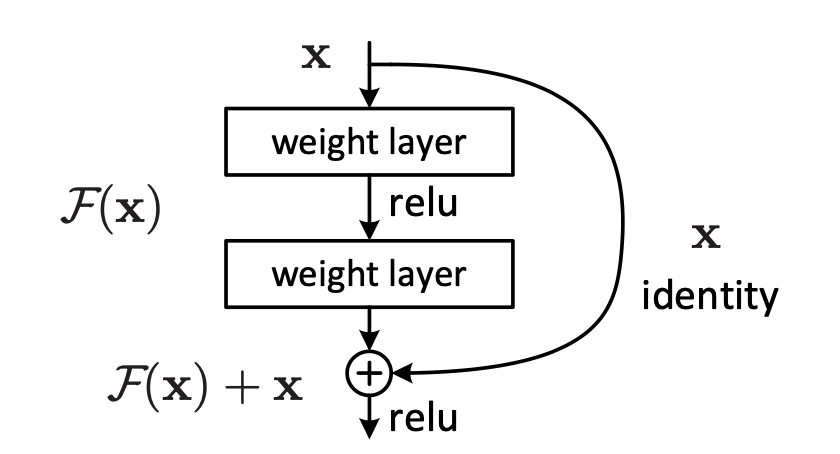
\includegraphics[width=130pt]{images/residual-block.png}
    \caption[Residual block]{Residual block \cite{resnet2016}}
    \label{fig:res-block}
\end{figure}

\begin{figure}[ht!]
    \centering
    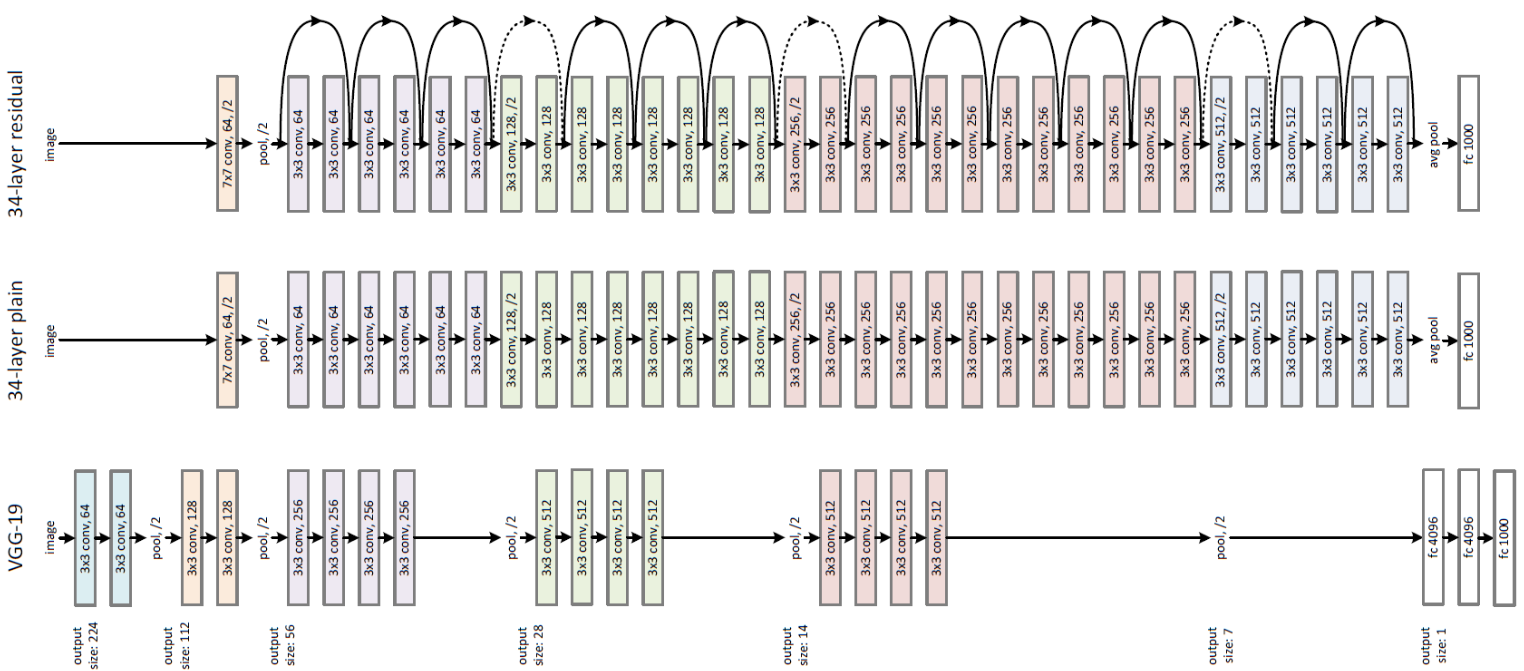
\includegraphics[width=350pt]{images/resnet.png}
    \caption[ResNet architecture]{ 34 layer ResNet (top), 34 layer plain network (middle), 19 layer VGG-19 (bottom)\cite{resnet2016}}
    \label{fig:resnet}
\end{figure}

\pagebreak